%IEEE template from https://www.overleaf.com/latex/templates/ieee-conference-template/grfzhhncsfqn
%Much template code eliminated.

%Report body is to be 4-10 pages EXCLUDING any reference and/or appendix
%pdf submission should be named "project_report.pdf"

\documentclass[conference]{IEEEtran}

%Leftover imports from the template. Most likely won't be needed.
\usepackage{amsmath}
\usepackage{amssymb,amsfonts}
%\usepackage{algorithmic}
%\usepackage{textcomp}
%\usepackage{xcolor}

\usepackage{graphicx}
\usepackage{comment}

\usepackage{listings} % Typeset Python
\lstset{breaklines=true,}

\usepackage[style=ieee]{biblatex}
\addbibresource{citations.bib}
\AtNextBibliography{\footnotesize}

\begin{document}

\title{COSC 5555-01 (22772) Spring 2023 Research Project: The effect of outpainting as a form of feature engineering on image classification}

\author{\IEEEauthorblockN{Michael Elgin}
\IEEEauthorblockA{\textit{University of Wyoming} \\
\textit{School of Computing}\\
Laramie, WY, USA\\
melgin@uwyo.edu}
\and
\IEEEauthorblockN{Long Tran}
\IEEEauthorblockA{\textit{University of Wyoming} \\
\textit{School of Computing}\\
Laramie, WY, USA \\
ltran2@uwyo.edu}
}

\maketitle

\clearpage %This is because we are supposed to have a cover page.

\section{Problem Statement}
% What is the problem that you are addressing?

Image classifiers suffer from misclassifications. The natural objective is to reduce the quantity of these by any way possible. Feature engineering has long been the focus of those seeking to improve model performance. With the recent advancement of image outpainting being available to the general public, we investigate the effect that outpainting as a form of feature engineering has on the
ability of an image dataset to make a classifier perform well.

In this project, we are testing and measuring the effectiveness of one particular implementation: a deep learning image-2-image program called Stable Diffusion for making new data for an image classifier.

Stable diffusion contains many text-to-image and image-to-image functions, of which outpainting falls into the image-to-image category. In this paper the CIFAR-10 dataset \cite{cifar} is used as a control group to train a classifier. Then outpainted images made from the same dataset are used to train a classifier of the same neural architecture. Then performance is compared to determine what merit outpainting may have as a form of feature engineering if it is done according to the methodology in this paper.

\section{Significance}
% What is the significance of your work? How your work adds to the body of the existing knowledge?

It would be good to see the impact that outpainted images created using Stable Diffusion have on the accuracy of a classifier. If the accuracy is not compromised, outpainting can open the door to techniques that produce synthetic data, thus allowing a larger amount of training samples and consequently improving model performance.

Publicly available image outpainting models are a recent advancement to the world. Not much is known about outpainting's potential to produce synthetic data. This ought to be explored because producing synthetic data for image training is far preferable to collecting data by human labor in terms of cost. Furthermore, the normal image augmentation techniques of rotation serve only to increase N by a factor of 4 assuming all of 90$^\circ$, 180$^\circ$, 270$^\circ$ are used, and 8 if those are all flipped horizontally and vertically as well. In the case of outpainting, N could be increased nearly without limit.

Image classifiers are increasingly becoming part of our world now that they are approaching human capability. With applications in self-driving cars and facial recognition, better classifiers can mean money is saved, time is saved, and lives are saved.

\section{Literature Survey}
% What has already been done? How your work is different than what has already been done in the literature?

Outpainting is an algorithm that extrapolates and extends existing images by inferring the missing regions using the known part of the image. In the past, almost all AIs use either autoregressive or diffusion models to generate images. 

Autoregressive models perform outpainting by dividing the desired output size into smaller units (called tokens, patches, …) and recursively generate each of those units, one at a time. Every unit generated will then become part of the input itself. Thus, the generation of the next unit will consider everything so far, including the newly generated portions, to fit into the “context” of the image as a whole. Wu et al. \cite{wu2022nuwainfinity} show an example of the ordering of outpainting in the following picture.

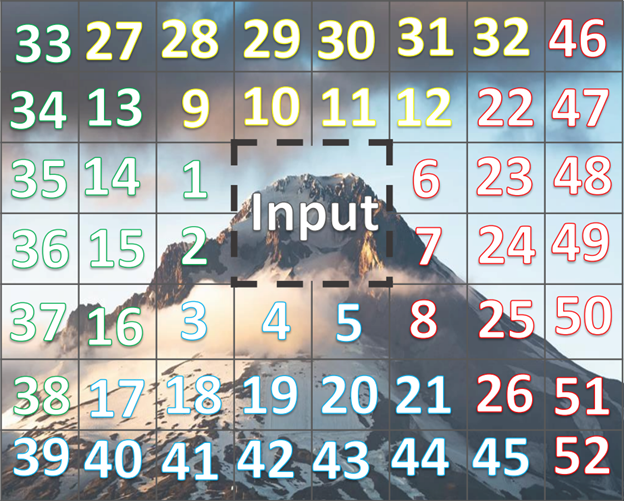
\includegraphics[scale=0.5]{autoregresive.png}

On the other hand, diffusion models work by going through what are called Forward/Reverse Diffusion processes. In the Forward Diffusion process, the models add noise to the image until it becomes “completely noisy”. Then, in the Reverse Diffusion process, the model learns to reconstruct the samples starting with complete noise, hence learning to create images similar to the original in the training dataset. Steins at \emph{medium} shows an example of this \cite{diffusionModel}.

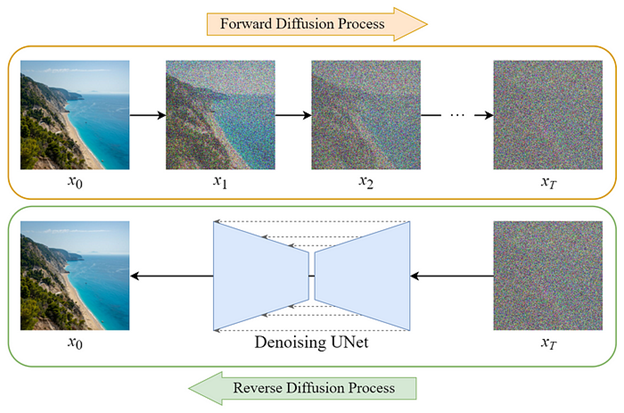
\includegraphics[scale=0.5]{diffusion.png}

Most of the research projects attempt to improve the accuracy of the outpainting process but few deals with finding out application of using these outpainted images. Singer et al. attempted to use constructed images (not outpainted) to create a 3D scene and even add time dimension, making a 4D animation. \cite[section 4.4.4]{singer2023textto4d}

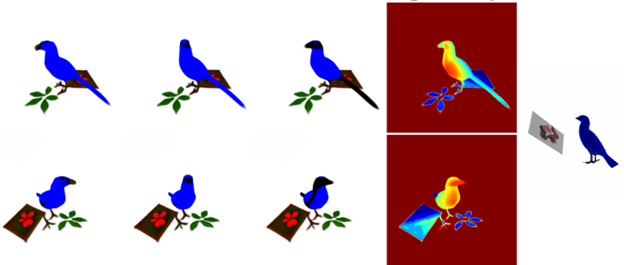
\includegraphics[scale=0.5]{Research.png}

Our research, while much simpler in nature, attempts to do something unique by researching other applications with these outpainted images. Specifically, we are using outpainted images to see whether they will be a good alternative as an augmentation, having equal footing to the original images as the input.

\section{Dataset Description}\label{dd}
% Detailed description of any dataset that you are using.

We used the famous CIFAR-10 dataset as our base, which consists of 60,000 32x32 color images in 10 classes. Thus, there are 6000 images per class, 5000 in training and 1000 in testing dataset.

Then, for the purpose of this project, we scaled down to using only 2 classes. We decided that using only 2 classes was sufficient to demonstrate the proof of concept. Additionally, it also affords the advantage of easier time with training the classifier models, as binary models are much easier to train and test compared to multi-classes ones. In the end, our initial dataset consists of 12,000 32x32 color images in 2 classes.

To create the second 64x64 dataset, we input all images mentioned in the previous section into Stable Diffusion model, creating a second dataset of the same size, which consists of 12,000 64x64 images in 2 classes. The outpainting was done with the following specifications.

\begin{center}
\begin{tabular}{|l|l|}
    \hline
    \textbf{Key} & \textbf{Value} \\
    \hline
    Checkpoint & v2-1\_768-ema-pruned.ckpt \\
    Checkpoint hash & [ad2a33c361] \\
    Resize mode & Just resize \\
    Sampling method & Euler a \\
    Sampling steps & 20 \\
    Width & 64 \\
    Height & 64 \\
    CFG scale (no prompt) & 7 \\
    Denoising strength & 0 \\
    Seed & 0 \\
    Script & Outpainting mk2 \\
    Pixels to expand & 8 \\
    Mask Blur & 1 \\
    Outpainting Directions & left, right, up, down \\
    Fall-off exponent & 1 \\
    Color variation & 0.05 \\
    \hline
\end{tabular}
\end{center}

\section{Methodology}
% What is your approach to solve the problem?

Our general approach is the following. First, our initial target was to obtain two different datasets, one natural and one synthetic. Then, we train two separate classifiers that take each of the two aforementioned datasets as input respectively, and evaluate them on testing datasets to obtain different metrics. We then use those  metrics to make conclusion on whether outpainted dataset increases, decreases or maintains the accuracy of the trained classifier. Finally, previous conclusions will help us answer the big question of whether outpainting will be a viable option as an augmentation technique.

First, to obtain the dataset, we downloaded the CIFAR-10 dataset from the official source. Then, we wrote a script in python, using pickle matplotlib libraries to read in the data, manipulate the binary to convert and save them as actual images.

Subsequently, we used Stable Diffusion v2.1 to outpaint all of the images in our original dataset in a batch to create the new outpainted dataset consisting of 12,000 64x64 color images.

Then, using Tensorflow and Keras, we trained a convolutional neural network model to classify the two labels from the original dataset. Our heuristic was to train a decent classifier with at least 90\% accuracy. As mentioned above, since we scaled down to only a binary classifier instead of a multi-classes one, we achieved this goal with ease. The model architecture follows.

\begin{lstlisting}[language=Python, basicstyle=\small]
model = Sequential()

model.add(Conv2D(32, (3, 3), padding='same', input_shape=inputShape))
model.add(Activation('relu'))
model.add(MaxPooling2D(pool_size=(2, 2)))
model.add(Dropout(0.25))

model.add(Flatten())
model.add(Dense(512))
model.add(Activation('relu'))
model.add(Dropout(0.5))
model.add(Dense(1))
model.add(Activation('sigmoid'))

model.compile(loss='binary_crossentropy',
                optimizer='adam',
                metrics=['accuracy'])
\end{lstlisting}

Finally, we run the model again using our new outpainted dataset as input, obtaining metrics such as True Positive, True Negative, False Positive, False Negative, and subsequently Accuracy, Precision and Recall, which helped guide us in making our final conclusions.

We measure the results of our classifiers in terms of its confusion matrix values, where $y$ represents the truth, and $\hat{y}$ represents the classifier's prediction.

$$
\text{True Positive (TP): }y = ship, \hat{y} = ship
$$
$$
\text{True Negative (TN): }y = horse, \hat{y} = horse
$$
$$
\text{False Positive (FP): }y = horse, \hat{y} = ship
$$
$$
\text{False Negative (FN): }y = ship, \hat{y} = horse
$$

These intermediate values allow us to calculate the remaining metrics:

$$
\text{Accuracy: }\frac{TP + TN}{TP + TN + FP + FN}
$$
$$
\text{Precision: }\frac{TP}{TP + FP}
$$
$$
\text{Recall: }\frac{TP}{TP + FN}
$$

\section{Results}
% By the end of the project, what have you accomplished?

It is first worth noting that the outpainted images were not quite as realistic as we had desired. Here an example of one of the worst results of an outpainted image, a horse picture in which the outpainting process completely failed to expand the sky, is shown.


\includegraphics{h132.png}
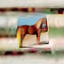
\includegraphics{h164.png}

This is contrasted with a better example in which color schemes connect properly for the most part even if the outpainted portion does not completely look like grass and a forest. Likewise the ships often had a much nicer expansion resembling water.


\includegraphics{h032.png}
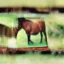
\includegraphics{h064.png}

\includegraphics{s032.png}
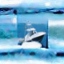
\includegraphics{s064.png}

The following confusion matrix shows the results of our classifier for size 32 images.

\begin{center}
\begin{tabular}{|c|c|}
  \hline
  TP = 960 & FN = 40 \\
  \hline
  FP = 28 & TN = 972 \\
  \hline
\end{tabular}
\end{center}

It therefore has the following metrics (among others):

\begin{itemize}
    \item Accuracy = .966
    \item Precision = .972
    \item Recall = .96
\end{itemize}

The following confusion matrix shows the results of our classifier for size 64 images.

\begin{center}
\begin{tabular}{|c|c|}
  \hline
  TP = 951 & FN = 49 \\
  \hline
  FP = 54 & TN = 946 \\
  \hline
\end{tabular}
\end{center}

It therefore has the following metrics (among others):

\begin{itemize}
    \item Accuracy = .948
    \item Precision = .946
    \item Recall = .951
\end{itemize}

\section{Challenges}
% Are there any challenges that you faced? Please describe what you did to mitigate the challenges. OR what changes you had to do to achieve the presented work. (You may address technical challenges or logistic challenges or both.)

The choice of the mask blur parameter was somewhat difficult. When it is set to 0, images are outpainted such that completely rigid line(s) are often formed between the original image and the outpainted section.

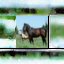
\includegraphics[]{h264-0.png}

However, as the mask blur increases, the original image progressively gets destroyed by the attempt to blur the new outpainted section with the original image.

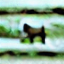
\includegraphics[scale=0.9]{h264-1.png}
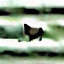
\includegraphics[scale=0.9]{h264-2.png}
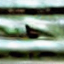
\includegraphics[scale=0.9]{h264-3.png}
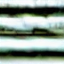
\includegraphics[scale=0.9]{h264-4.png}

This was a situation where there was no good answer, only trade-offs. We settled on a Mask blur of 1.

A second challenge was outpainting without a prompt. Image-to-image processes in Stable Diffusion, in addition to the text-to-image processes, are designed to be text-guided. This experiment performed the outpainting without any text prompt. Doing so most likely would have had a positive effect and will be discussed in section \ref{conc}.

A third challenge was the original size of the image for outpainting. A 32x32 image does not give very much pixel context compared to larger resolution images. That paired with the absence of a text prompt led to some very strange (and ultimately unrealistic) outpainted images. With this in mind, no matter how the parameters in section \ref{dd} were varied from what they are currently listed as, things only got worse.

A fourth challenge was the selection of model architecture. It seemed desirable to stay away from a state-of-the-art convolutional architecture because it might be difficult to discern differences among classifiers whose accuracy on CIFAR-10 was already on the order of 99\%, however at the same time there was definitely a need for a model that was strong enough to keep sufficiently away from the random-baseline guessing of 50\%. Ultimately we decided to start with an example model and remove layers and adjust it until reaching an accuracy of about 90\% on the size 32 data.

A fifth challenge was how to load all of the outpainted data in a format that could be fed to a Keras model. The CIFAR-10 dataset and the accompanying tutorials do not have the data formatted as a series of .png files inside a directory, though after creating the outpainted images from Stable Diffusion we were forced to load the outpainted data from this format. Fortunately after some searching, it was discovered that Tensorflow has some handy functions for building an iterable training object from a folder of png files. The following is an excerpt of our solution in load\_data.py, our file to load the .png file data into classifier.py

\begin{lstlisting}[language=Python, basicstyle=\tiny]
#Create a list of file paths for all png images in the directory
file_paths = tf.io.gfile.glob(image_dir + "/*.png")

#Sort - otherwise they don't stay in sync with labels
file_paths = sorted(file_paths, key=lambda x: int(x.split("\\")[-1].split(".")[0]))

#Create a TensorFlow dataset from the file paths
dataset = tf.data.Dataset.from_tensor_slices(file_paths)
\end{lstlisting}

\section{Conclusions}\label{conc}
% Present a summary of your work and draw conclusions (if any).

The results obtained were not what we expected. We believed that outpainting would have a slight positive effect on the accuracy, precision, and recall of a classifier. Instead, there was a slight \emph{decrease} on the accuracy, precision, and recall.

CNN accuracy most likely has more to do with the object in frame, such as a horse or a ship, than any influence the background may have. CNNs appear to be more shape sensitive than color sensitive due to their kernel convolutions. In the case of the size 32 (normal) cifar-10 images, the image is almost always completely shown in the image i.e. the entire horse or entire ship was in frame and there was nothing left of it to expand. Furthermore, it's entirely possible that outpainting in a sense serves as a ``distraction" to the classifier rather than giving it context to help it predict properly. It may have been a human bias that there was an expectation that this surrounding context might help in classification. To imagine this, consider that if a human were to be shown the outpainted portion of one of the images, but had the original center missing, it would be very easy for the human to still guess horse or ship correctly because a human can easily make a judgement related to the shape of trees in the background or waves of the ocean, or even the mere pixel colors of green/brown vs blue. However, CNNs are not looking at the real world this way. They are convolving a filter that matches a shape. So even if outpainting creates a background that resembles the continuation of a green pasture, a forest, or the waves of the ocean, this is not necessarily helpful because the CNN doesn't know what any of those things are. Worse still, since those outpainted images are merely labeled horse or ship, there is the risk that it is learning that those trees or waves \emph{are} the horse or the ship. For this reason it may be the case that machine-learning based on outpainted images is not only not helpful, but outright harmful because it takes focus away from the horses and ships by giving them a background of objects that are neither.

Even though the metrics were slightly worse on the size 64 (outpainted) classifier, this approach \emph{does} potentially still have merit because of the sheer volume of augmented training data that can be produced from outpainting. As an example, consider the possibility of not merely duplicating the training set to also be size 10,000 for the outpainted classifier, but rather 100,000, or 1,000,000. At this scale it is likely that an improvement would be seen. The reason N was kept the same for both classifiers is that the effect of outpainting would be most precisely determined if as many variables as possible were kept the same.

Since outpainted data can give quite good performance for a classifier, data augmented by outpainting will likely serve a role as a ``supplement" to the original training data of a classifier, not a replacement of it. In this sense it would be considered a similar data augmentation tool as the rotations and flips mentioned earlier in this paper.

\subsection{Future work}

The first avenue of future work to consider is that of running more training epochs over the classifiers. These models were trained on a laptop, so the amount of compute that could be performed was fairly limited. It would be an interesting experiment to see how the performance of 10 epochs of 10,000 32 images compares to the performance of 100,000 outpainted images all of which are different, most likely done by incrementing the random number seed by 1 for each batch of 10,000.

In regards to outpainting with a text prompt, it would be a good idea to re-run this experiment with the following modification: first, sort the original size 32 horses and ships into separate folders, then perform the outpainting in a batch with each batch having the text guidance of ``horse" and ``ship" respectively. More deluxe text prompts might be even more helpful, but would be cost prohibitive in terms of labor to tailor a unique prompt to every single image in a size 10,000 training set.

The third change to explore would be different datasets than CIFAR-10. ImageNet contains images of a much larger size, so they may very well serve as a better basis for outpainting than CIFAR-10 did. Such an experiment would be contingent upon access to more compute.

Lastly, multi-class classification is another potential route to explore, though this experiment has not given reason to believe any different conclusions would be drawn. In any case the possibility is still there.

\section{Possible Venue(s)}
% What are the suitable venues where your work can be shared? For example, you could mention a conference where you may want to present your work.

While we acknowledge the so called ``top tier" AI conferences such as ICML, ICLR, AAAI, NeurIPS, etc., we feel most comfortable submitting papers only to conferences we have been to before. Michael Elgin has only attended AGI-22 in Seattle. That conference consisted of several lightning rounds of papers. AGI-23 is scheduled to be in Stockholm though there are no plans at this time to attend, and it feels like submitting a paper would come with the expectation of attendance, even if only virtually.

Furthermore, consideration of submission should, in our opinion, be contingent upon a working proof-of-concept i.e. that we discovered something worthwhile, not merely confirmed that something didn't work very well.

\section{Contributions}
% What contributions are made by each of the team members to achieve the presented work.

\subsection{Michael Elgin}
\begin{enumerate}
    \item LaTeX base code
    \item Image outpainting via Stable Diffusion
    \item Proposal text (concurrently)
    \item data\_preprocess.py
    \item load\_data.py
    \item Report sections
    \begin{enumerate}
        \item Possible Venues
        \item Problem Statement
        \item Results
        \item Conclusions
    \end{enumerate}
\end{enumerate}

\subsection{Long Tran}
\begin{enumerate}
    \item Proposal text (concurrently)
    \item classifier.py
    \item Report sections
    \begin{enumerate}
        \item Significance
        \item Literature Survey
        \item Dataset description
        \item Methodology
    \end{enumerate}
\end{enumerate}

\printbibliography

\end{document}